\documentclass[journal,12pt,twocolumn]{IEEEtran}

\usepackage{setspace}
\usepackage{gensymb}

\singlespacing


\usepackage[cmex10]{amsmath}

\usepackage{amsthm}

\usepackage{mathrsfs}
\usepackage{txfonts}
\usepackage{stfloats}
\usepackage{bm}
\usepackage{cite}
\usepackage{cases}
\usepackage{subfig}

\usepackage{longtable}
\usepackage{multirow}

\usepackage{enumitem}
\usepackage{mathtools}
\usepackage{steinmetz}
\usepackage{tikz}
\usepackage{circuitikz}
\usepackage{verbatim}
\usepackage{tfrupee}
\usepackage[breaklinks=true]{hyperref}
\usepackage{graphicx}
\usepackage{tkz-euclide}
\usepackage{float}

\usetikzlibrary{calc,math}
\usepackage{listings}
    \usepackage{color}                                            %%
    \usepackage{array}                                            %%
    \usepackage{longtable}                                        %%
    \usepackage{calc}                                             %%
    \usepackage{multirow}                                         %%
    \usepackage{hhline}                                           %%
    \usepackage{ifthen}                                           %%
    \usepackage{lscape}     
\usepackage{multicol}
\usepackage{chngcntr}

\DeclareMathOperator*{\Res}{Res}

\renewcommand\thesection{\arabic{section}}
\renewcommand\thesubsection{\thesection.\arabic{subsection}}
\renewcommand\thesubsubsection{\thesubsection.\arabic{subsubsection}}

\renewcommand\thesectiondis{\arabic{section}}
\renewcommand\thesubsectiondis{\thesectiondis.\arabic{subsection}}
\renewcommand\thesubsubsectiondis{\thesubsectiondis.\arabic{subsubsection}}


\hyphenation{op-tical net-works semi-conduc-tor}
\def\inputGnumericTable{}                                 %%

\lstset{
%language=C,
frame=single, 
breaklines=true,
columns=fullflexible
}
\begin{document}


\newtheorem{theorem}{Theorem}[section]
\newtheorem{problem}{Problem}
\newtheorem{proposition}{Proposition}[section]
\newtheorem{lemma}{Lemma}[section]
\newtheorem{corollary}[theorem]{Corollary}
\newtheorem{example}{Example}[section]
\newtheorem{definition}[problem]{Definition}

\newcommand{\BEQA}{\begin{eqnarray}}
\newcommand{\EEQA}{\end{eqnarray}}
\newcommand{\define}{\stackrel{\triangle}{=}}
\bibliographystyle{IEEEtran}
\providecommand{\mbf}{\mathbf}
\providecommand{\pr}[1]{\ensuremath{\Pr\left(#1\right)}}
\providecommand{\qfunc}[1]{\ensuremath{Q\left(#1\right)}}
\providecommand{\sbrak}[1]{\ensuremath{{}\left[#1\right]}}
\providecommand{\lsbrak}[1]{\ensuremath{{}\left[#1\right.}}
\providecommand{\rsbrak}[1]{\ensuremath{{}\left.#1\right]}}
\providecommand{\brak}[1]{\ensuremath{\left(#1\right)}}
\providecommand{\lbrak}[1]{\ensuremath{\left(#1\right.}}
\providecommand{\rbrak}[1]{\ensuremath{\left.#1\right)}}
\providecommand{\cbrak}[1]{\ensuremath{\left\{#1\right\}}}
\providecommand{\lcbrak}[1]{\ensuremath{\left\{#1\right.}}
\providecommand{\rcbrak}[1]{\ensuremath{\left.#1\right\}}}
\theoremstyle{remark}
\newtheorem{rem}{Remark}
\newcommand{\sgn}{\mathop{\mathrm{sgn}}}
\providecommand{\abs}[1]{\vert#1\vert}
\providecommand{\res}[1]{\Res\displaylimits_{#1}} 
\providecommand{\norm}[1]{\lVert#1\rVert}
%\providecommand{\norm}[1]{\lVert#1\rVert}
\providecommand{\mtx}[1]{\mathbf{#1}}
\providecommand{\mean}[1]{E[ #1 ]}
\providecommand{\fourier}{\overset{\mathcal{F}}{ \rightleftharpoons}}
%\providecommand{\hilbert}{\overset{\mathcal{H}}{ \rightleftharpoons}}
\providecommand{\system}{\overset{\mathcal{H}}{ \longleftrightarrow}}
	%\newcommand{\solution}[2]{\textbf{Solution:}{#1}}
\newcommand{\solution}{\noindent \textbf{Solution: }}
\newcommand{\cosec}{\,\text{cosec}\,}
\providecommand{\dec}[2]{\ensuremath{\overset{#1}{\underset{#2}{\gtrless}}}}
\newcommand{\myvec}[1]{\ensuremath{\begin{pmatrix}#1\end{pmatrix}}}
\newcommand{\mydet}[1]{\ensuremath{\begin{vmatrix}#1\end{vmatrix}}}
\numberwithin{equation}{subsection}
\makeatletter
\@addtoreset{figure}{problem}
\makeatother
\let\StandardTheFigure\thefigure
\let\vec\mathbf
\renewcommand{\thefigure}{\theproblem}
\def\putbox#1#2#3{\makebox[0in][l]{\makebox[#1][l]{}\raisebox{\baselineskip}[0in][0in]{\raisebox{#2}[0in][0in]{#3}}}}
     \def\rightbox#1{\makebox[0in][r]{#1}}
     \def\centbox#1{\makebox[0in]{#1}}
     \def\topbox#1{\raisebox{-\baselineskip}[0in][0in]{#1}}
     \def\midbox#1{\raisebox{-0.5\baselineskip}[0in][0in]{#1}}
\vspace{3cm}
\title{Assignment 9}
\author{Satya Sangram Mishra}
\maketitle
\newpage
\bigskip
\renewcommand{\thefigure}{\theenumi}
\renewcommand{\thetable}{\theenumi}
Download all python codes from 
\begin{lstlisting}
https://github.com/satyasm45/Summer-Internship/tree/main/Assignment-9/Codes
\end{lstlisting}
%
and latex-tikz codes from 
%
\begin{lstlisting}
https://github.com/satyasm45/Summer-Internship/tree/main/Assignment-9/Codes
\end{lstlisting}
%
\section{Question No. 2.56}
Solve:  x-2y $\leq$ 3, 3x+4y $\geq$ 12, x $\geq$ 0, y $\geq$ 1.
\section{Explanation}
\begin{enumerate}
    \item Solving first pair of inequality:
    \begin{align}
\label{eq:line_two_ineq}
\begin{split}
    -x+2y &\geq -3
\\
    3x+4y &\geq 12
\end{split}
\end{align}
\solution  Let $u_1 \ge 0, u_2 \ge 0$.  This may be expressed as
\begin{align}
\vec{u} = \myvec{u_1\\u_2}\succeq \vec{0}
\end{align}
%
\eqref{eq:line_two_ineq} can then be expressed as
\begin{align}
\myvec{-1 & 2 \\ 3 & 4}\vec{x}  &\succeq \myvec{-3\\12}
\\
\myvec{-1 & 2 \\ 3 & 4}\vec{x}  -\vec{u}&=\myvec{-3\\12}
\\
\text{or, }
\myvec{-1 & 2 \\ 3 & 4}\vec{x} &= \myvec{-3\\12} +\vec{u}
\end{align}
%
resulting in 
\begin{align}
\vec{x} &= \myvec{-1 & 2 \\ 3 & 4}^{-1}\myvec{-3\\12} +\myvec{-1 & 2 \\ 3 & 4}^{-1}\vec{u}
\\
\text{or, } \vec{x} &= \myvec{3.6\\0.3} +\frac{-1}{10}\myvec{4 & -2 \\ -3 & -1}\vec{u}\label{eq:1}
\end{align}
    
    \item Similarly,Solving second pair of inequality:
    \begin{align}
\label{eq:line_two_ineq}
\begin{split}
    x\geq 0
\\
    y \geq 1
\end{split}
\end{align}
\solution  Let $u_1 \ge 0, u_2 \ge 0$.  This may be expressed as
\begin{align}
\vec{u} = \myvec{u_1\\u_2}\succeq \vec{0}
\end{align}
%
\eqref{eq:line_two_ineq} can then be expressed as
\begin{align}
\myvec{1 & 0 \\ 0 & 1}\vec{x}  &\succeq \myvec{0\\1}
\\
\myvec{1 & 0 \\ 0 & 1}\vec{x}  -\vec{u}&=\myvec{0\\1}
\\
\text{or, }
\vec{x} &= \myvec{0\\1} +\vec{u}\label{eq:2}
\end{align}
\end{enumerate}
From \eqref{eq:1} and \eqref{eq:2},solution of the given system of inequalities can be found out graphically by intersection as shown by the below figures generated by Python:

As seen from \ref{fig:inequality3} the solution region is bounded by line segments AB and BC and the line x-2y=3.Beyond A the region expands infinitely along the Y axis,Beyond C the region includes all the portion above the line x-2y=3.

Also Point D shows the importance of $\myvec{3.6\\0.3}$ derived in \eqref{eq:1}

\numberwithin{figure}{section}
\begin{figure}[!ht]
\centering
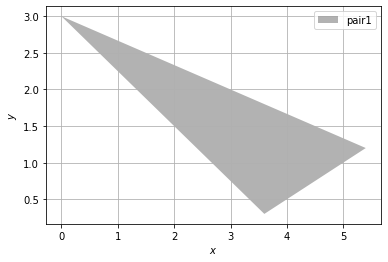
\includegraphics[width=\columnwidth]{Figure9_1}
\caption{Inequality pair 1}
\label{fig:inequalities1}	
\end{figure}
\numberwithin{figure}{section}
\begin{figure}[!ht]
\centering
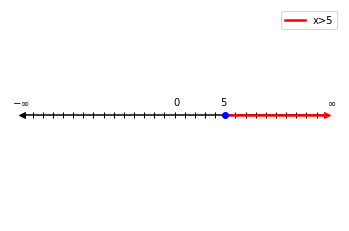
\includegraphics[width=\columnwidth]{Figure9_2}
\caption{Inequality pair 2}
\label{fig:inequalities2}	
\end{figure}
\numberwithin{figure}{section}
\begin{figure}[!ht]
\centering
\includegraphics[width=\columnwidth]{Figure9_3}
\caption{Intersection of \ref{fig:inequalities1} and \ref{fig:inequalities2}}
\label{fig:inequality3}	
\end{figure}
The common region shown by \ref{fig:inequality3} is the solution of set of inequalities.
\end{document}
